\newcommand{\package}{\emph}
\chapter{Introduction}
Solar energy is one of the key alternative energy sources. The recent developments in solar panels and different business models around them made the photo-voltaic(PV) power plants more economical. However, the variability in PV output power make the integration into main energy grid risky and slow\cite{solar_variable}. These fluctuations come from cloud states in sky, and it has two different effects, one decreasing the power, the other one increasing the power. Firstly, if the clouds cover the sun completely or partially, some area of plant is shadowed and does not receive direct sunlight, causing a power drop. On the other hand, if the clouds are not occluding the the sun completely or at all, based on their type, height, position and time, they can re-reflect some part of the irradiation\footnote{Irradiation is the sum of irradiance over a time period, expressed in $Wh/m^2$} which is reflected by ground, back into the power plant. In this case, the input irradiance\footnote{Irradiance is understood as instantaneous density of solar radiation incident on a given surface, typically expressed in $W/m^2$} and consequently the output power increases. In the electricity grid, the stability of power is vital. Therefore, if we want to integrate a PV power source into the grid we need to compensate for any power drop by using other electricity sources, and also restrain any excessive power. That is why we need to predict these short-time power changes in advance to design better strategies for handling them and ultimately provide a guaranteed stable power in the grid. In this chapter, we first explain different approaches towards this prediction problem, then we describe overview of the setup used in this study, and finally we talk about accuracy metrics for the result. 


\section{Power prediction approaches for a PV plant}
\label{sec:overview}
The large variety of cloud characteristics such as motion, height, opacity and spatial distribution makes the cloud-induced fluctuations difficult to predict. However, according to these comprehensive surveys\cite{survay1, survay2}, solar irradiance forecasting techniques have been successfully developed. 
These include numerical weather models (NWPs)\cite{nwp13} using pattern recognition of meteorological data for irradiance prediction, satellite-based forecasts using cloud motion vectors to determine sun occlusion based on fixed velocity model and predict power \cite{sat_based13,sat_based2004, sat_based99}, statistical methods based on machine learning applied on past several years trend\cite{stat_based13} and time series analysis\cite{time_serise09}
which are mostly developed for intra-day and day-ahead forecasts. However, for very short-term power prediction applications, the interest horizon stretches up to 30 minutes ahead. And therefore, these methods fall behind the required spatial or temporal resolution required on cloud-induced irradiance variability\cite{survay1}.

\subsection{Ground whole-sky imagery}
For achieving this high resolution forecasts, vision-based methods using total-sky-cameras are developed. The earliest works use cameras for monitoring cloud cover characteristics\cite{cloud_cover03, cloud_cover08} and aerosol properties\cite{areosal1, areosal2}. In recent years, using sky cameras for solar irradiance forecast has grown rapidly and several successful works have been developed by analyzing motion, optical and distribution of clouds in the whole-sky images captured by a fisheye lens camera (\cite{cloud_detection_using_RBR, cloud_height14, point_forecast14}). 
Using only one camera for data input, some methods\cite{point_forecast14} predict sun occlusions perceived by the camera and therefore, their forecast in only valid for the point very close to the camera, since areas further away might be sunny or cloudy and camera's point of view is not covering that area. However, one can incorporate cloud base height to calculate projection of clouds shadows on the ground. This information is usually acquired by using a laser based cloud base sensor (ceilometer) and make the area irradiance forecasts more accurate\cite{cloud_height14}. It is theoretically possible to use two or more cameras in the site mounted with a distance about 50m and by applying stereo algorithm, find the cloud height; however, this method has not been investigated in practice yet. In this research we focus on ground whole-sky imagery methods aimed for very short-term irradiance forecast.

%\section{Data acquisition setup}
%This study uses the data from a PV plant in Cavriglia area in Italy.
%The setup for this study is based on one sky camera with fisheye lense mounted at the top of the building right next to the PV plant. This type of camera with 180 degree area of view gives us the whole sky in one image. Furthermore, there are two irradiance sensors-Pyranometer) located at the same location as camera, one with the same angle as solar panels-which is tilted about 40 degrees towards the south- and the other one about 40 degrees tilted about 35 degrees towards the north. The data acquisition software takes several images with different exposures every 6 seconds and combine them to get HDR images. The irradiance sensor measurements and temperature are also recorded at the same intervals. Finally, we record power output of PV plant every 3 seconds.

\section{Cloud segmentation, cloud tracking}
For predicting the future state of clouds in the sky we need to first know where the clouds are. This is done by applying a dynamic-threshold segmentation algorithm on red to blue channel ratio of RGB images. Several studies has shown that the red to blue ratio is a good criterion for cloud segmentation, but the threshold for this ratio should be set in a way that discriminate clouds locally but be smooth globally. For this purpose, image pixels are mapped to a grid and threshold is determined for each grid separately while maintaining the smoothness globally. This method handles cloud color variation for different cloud types very well. This detail of the algorithm for finding this optimal thresholds for every grid is out of the scope of this study. One sample result of such segmentation is given in Figure \ref{fig:cloud_seg}.
\begin{figure}[h]
\caption{Cloud segmentation sample}
\label{fig:cloud_seg}
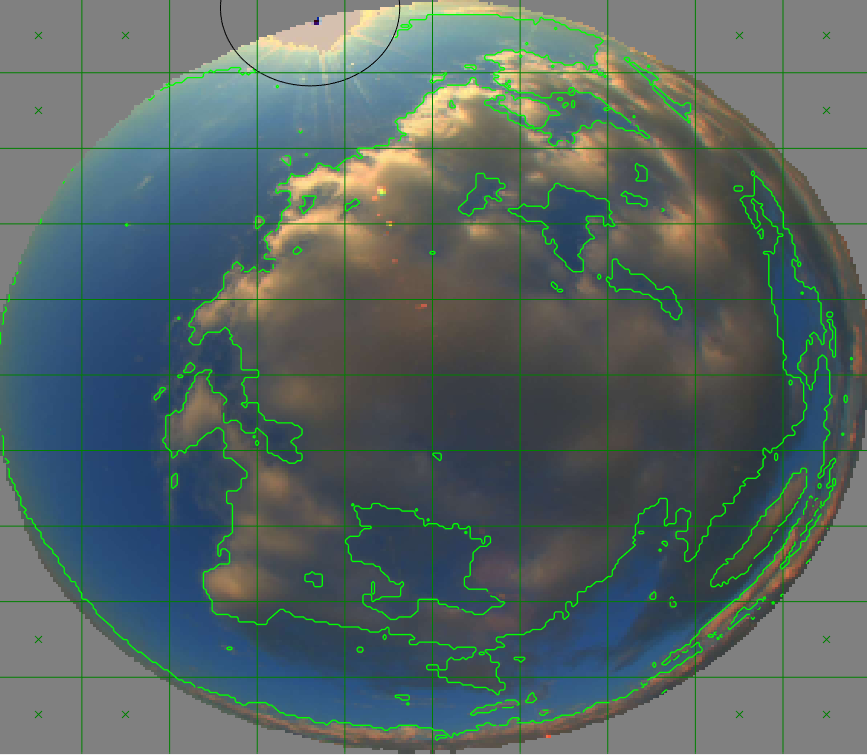
\includegraphics[scale=.4]{cloud_segment2}
\centering
\end{figure}

This is a binary segmentation, meaning that classification result for every pixel is either cloud or not cloud (i.e. sky). If sun is visible in the image, a small circle around the sun is excluded for segmentation, thus does not have any class in the output. The same goes for pixels outside of sky mask. After detecting the clouds in a sequence of images, we can apply optical flow algorithm on some points of interest in the first image and extract the cloud movement as motion vectors of optical flow. This cloud tracking pipeline gives us the clouds position is the sky for very short time in future. The result of experiment on several future time horizon has shown that accuracy decreases considerably after 30 minutes, especially in high speed cloud motions.

\section{Image irradiance estimation for power prediction}
The final step in power prediction is to associate a potential power estimate to any time in several minutes ahead knowing the cloud positions and their characteristic in that time. The generated power of a PV plant depends on several factors including received irradiance, operational temperature and panels’ specification. However, the only factor which changes rapidly and has a huge impact on the output power is irradiance. Therefore, in our power prediction framework, we use a power prediction adaptation method with recorded data of previous minutes to derive the power output from future irradiance estimations. The scaling factor for the result is calculated by diving the recorded power output and irradiance sensor measurements. Thus, this power adaptation mechanism, separates and defines our main problem as estimating the received irradiance from a clouds attributes in a specific time and location.

\section{Irradiance components}
The total solar radiation -GHI\footnote{Global Horizontal Irradiation}- which hits the surface of solar panels consists of three basic components, direct -DNI\footnote{Direct Normal Irradiance}-, diffuse -DHI\footnote{Diffuse Horizontal Irradiance}- and reflected. The direct part comes from the sunlight beams directly raying from sun direction to the solar module. While passing through atmosphere, some amount of sunlight scatters in every direction by dense particles. The portion of this scattered light which hits the module forms the diffuse irradiation for solar panels. 
Reflected irradiance represents sunlight that is reflected off the clouds or ground around the array of panels. The source of this reflected radiation can be DNI or DHI. Rate of the reflection depends on clouds coverage, size of the ground that is visible from the module and their albedo coefficient\footnote{The portion of the incident irradiance that is reflected}. The albedo coefficient for ground is typically 0.2, though it can be higher during snowy periods in cold climates. The albedo coefficient for clouds depends on their type, density, temperature and etc. These components are shown in figure \ref{fig:irr_comps}

\begin{figure}[h]
\caption{Irradiance components}
\label{fig:irr_comps}
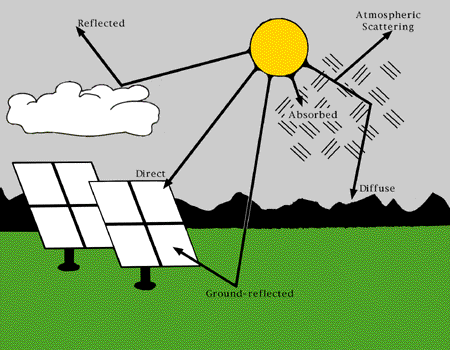
\includegraphics[scale=.7]{irr_components}
\centering
\end{figure} 

Total irradiation is related to other three components with this formula:
\[ GHI = DNI \times cos (Z) + DHI + reflected \]
where Z is the solar zenith angle-the angle between the direction of the sun and the line directly overhead.
Since distinguishing between the reflected and diffuse irradiation is practically hard and also there is not any ground truth value for training, we decided to combine both of them as the diffuse component. Thus, the formula changes to:
\begin{equation}
\label{eq:irr_components}
GHI = DNI \times cos (Z) + DHI
\end{equation}
where DHI is sum of all non-direct irradiations.

\section{Accuracy metric}
For measuring accuracy of the result we can use popular error measure of RMSE-Root Mean Square Error which is defined in Eq. \ref{eq:rmse_eq1}.

\begin{equation}
\label{eq:rmse_eq1}
RMSE = \sqrt{\frac{\sum_{i=1}^{n}{(DHI_{observed, i} - DHI_{estimated ,i})^2}}{n}}
\end{equation}
where $n$ is the number of samples. This choice makes sense for our application, plus it enables us to compare our results to other related works or vice versa.

\section{Thesis structure}
This thesis organized in six chapters. In First chapter, we give in introduction to the PV plant power prediction pipeline and describe how the result of this study will be used in a power prediction system. In chapter \ref{sec:related_work_chapter}, we do a quick survey on related works which have a focus on irradiance estimation from sky images. Then, our approach, dataset and algorithms for tackling this problem are explained in chapter \ref{sec:my_work_chapter}. Afterwards, we show the result of our method on the dataset in chapter \ref{sec:result_chapter} and discuss the performance of different configurations using images. In chapter \ref{sec:future_work_chapter} some possible future improvements on this topic are mentioned. And finally the thesis is concluded in chapter \ref{sec:conclusion_chapter}.
%However, since there are not any other publicly available study on this specific problem to compare our RMSE with, we can define our own error measures which quantify our solution quality better. For example, apart from RMSE, we calculate a relative error as well that penalize errors for irradiances higher than a specific value more. And errors for irradiances lower than that value, will be penalized less. This cutting value is set as 100 and the scale is logarithmic, because when the irradiance is less than 100, the power output of plant is very low and practically not useful in grid. On the other hand, we want more precise result for very high irradiances. This means errors for small irradiances are less important than errors in big big ones. We also use MBE (mean bias error) and $R^2$ for correlation coefficient.